\documentclass[aspectratio=169,10pt]{beamer}

\usepackage[utf8]{inputenc}
\usepackage[T1]{fontenc}
\usepackage[shorthands=off, turkish]{babel}
\usepackage{amsmath,amssymb,amsfonts}
\usepackage{graphicx}
\graphicspath{{figures/}{./}}
\usepackage{booktabs}
\usepackage{tabularx}
\usepackage{array}

% --- IEEE Conference Presentation Theme & Colors ---
\usetheme{Madrid}
\usecolortheme{whale}
\definecolor{IEEEBlue}{RGB}{0, 98, 155}
\definecolor{IEEENavy}{RGB}{0, 40, 85}
\definecolor{IEEEGray}{RGB}{242, 245, 248}

\setbeamercolor{palette primary}{bg=IEEENavy,fg=white}
\setbeamercolor{palette secondary}{bg=IEEEBlue,fg=white}
\setbeamercolor{palette tertiary}{bg=IEEENavy,fg=white}
\setbeamercolor{structure}{fg=IEEEBlue}
\setbeamercolor{title}{bg=IEEENavy,fg=white}
\setbeamercolor{frametitle}{bg=IEEENavy,fg=white}
\setbeamercolor{block title}{bg=IEEEBlue,fg=white}
\setbeamercolor{block body}{bg=IEEEGray,fg=black}
\setbeamertemplate{navigation symbols}{}
\setbeamertemplate{caption}[numbered]

\title[IEEE Ara Sunum --- Deep Learning]{Önceden Eğitilmiş Türkçe Modellerle İnce Ayar (Fine-Tuning) Tabanlı Chatbot Geliştirme ve Seq2Seq Karşılaştırmalı Başarım Analizi}
\subtitle{Ara Sunum (Midterm Presentation) --- IEEE Akademik Formatı}
\author[Seyit Ali Arslan (240711024)]{\textbf{Seyit Ali Arslan} \\ Öğrenci No: 240711024}
\institute[Atatürk Üniversitesi]{Yapay Zeka ve Veri Mühendisliği Bölümü\\Atatürk Üniversitesi, Erzurum, Türkiye\\Ders: Deep Learning (2026--2027)}
\date{Kasım 2026}

\begin{document}

% --- SLAYT 1: Kapak ---
\begin{frame}
    \titlepage
\end{frame}

% --- SLAYT 2: İçindekiler ---
\begin{frame}{Sunum Akışı (IEEE Bölümlendirmesi)}
    \begin{columns}[T]
        \begin{column}{0.48\textwidth}
            \begin{block}{I--IV. Teorik Çerçeve ve Veri}
                \begin{itemize}
                    \item \textbf{I. Giriş ve Problem Tanımı:} Sondan eklemeli Türkçe morfolojisi ve Seq2Seq darboğazı
                    \item \textbf{II. Motivasyon:} Sıfırdan Eğitim vs. Transfer Öğrenme (Fine-Tuning)
                    \item \textbf{III. Veri Kümesi ve EDA:} 50.000 Türkçe Diyalog Çifti (\%80 / \%10 / \%10)
                    \item \textbf{IV. Metodoloji:} Tokenizasyon, AdamW ve Kayıp Maskeleme
                \end{itemize}
            \end{block}
        \end{column}
        \begin{column}{0.48\textwidth}
            \begin{block}{V--VIII. Modeller ve Deneysel Bulgular}
                \begin{itemize}
                    \item \textbf{V. Temel Model (Baseline):} 2-Katmanlı Seq2Seq Bi-LSTM + Bahdanau Attention
                    \item \textbf{VI. Model 1:} Önceden Eğitilmiş \texttt{Turkish-GPT-2} İnce Ayarı (124.4M)
                    \item \textbf{VII. Deneysel Karşılaştırma:} Loss, Perplexity (PPL), BLEU, ROUGE ve Latency (ms)
                    \item \textbf{VIII. Nitel Çıktılar ve Final Planı (LoRA)}
                \end{itemize}
            \end{block}
        \end{column}
    \end{columns}
\end{frame}

% --- SLAYT 3: Giriş, Problem Tanımı ve Motivasyon ---
\begin{frame}{I. Giriş ve Problem Tanımı \& II. Motivasyon}
    \begin{columns}[T]
        \begin{column}{0.48\textwidth}
            \begin{block}{I. Problem Tanımı}
                \begin{itemize}
                    \item \textbf{Sondan Eklemeli (Agglutinative) Yapı:} Türkçede kök + yapım/çekim ekleri kelime dağarcığını üstel büyütür ve \textbf{OOV (Out-of-Vocabulary)} sorununa yol açar.
                    \item \textbf{Seq2Seq RNN/LSTM Sınırları:} Sıralı (\textit{sequential}) işleme nedeniyle uzun cümlelerde \textbf{darboğaz (bottleneck)} ve bağlam kaybı yaşanır; GPU paralelleştirmesi sınırlıdır.
                \end{itemize}
            \end{block}
        \end{column}
        \begin{column}{0.48\textwidth}
            \begin{block}{II. Motivasyon ve Çözüm Yaklaşımı}
                \begin{itemize}
                    \item \textbf{Transfer Öğrenme (Fine-Tuning):} Büyük Türkçe derlemlerde önceden eğitilmiş Transformer ağırlıklarını diyalog alanına aktarmak eğitim maliyetini düşürürken dilbilgisel kavrayışı korur.
                    \item \textbf{Deneysel Kıyaslama:} Klasik 2-katmanlı \textbf{Seq2Seq Bi-LSTM + Bahdanau Attention} ile \textbf{Fine-Tuned Turkish-GPT-2} somut metriklerle kıyaslanmıştır.
                \end{itemize}
            \end{block}
        \end{column}
    \end{columns}
\end{frame}

% --- SLAYT 4: Veri Kümesi ve Bölümleme ---
\begin{frame}{III. Veri Kümesi ve Veri Bölümleme (\%80 / \%10 / \%10)}
    \begin{columns}[c]
        \begin{column}{0.44\textwidth}
            \begin{block}{Veri Önişleme Boru Hattı}
                \begin{itemize}
                    \item \textbf{Kaynaklar:} Hugging Face Türkçe diyalog kümeleri (\texttt{Ba2han/Turkish\_Chat}, \texttt{AEG/Turkish-Chat-62k}, \texttt{yeniguno/turkish-chatbot-data}).
                    \item \textbf{Temizleme:} HTML, Markdown kalıntıları, bozuk karakterler ve mükerrer kayıtlar elendi.
                    \item \textbf{Toplam Boyut:} \textbf{50.000} filtrelenmiş doğal Türkçe diyalog çifti (2--45 kelime).
                    \item \textbf{Bölümleme:} \textbf{40.000} Train (\%80), \textbf{5.000} Val (\%10), \textbf{5.000} Test (\%10).
                \end{itemize}
            \end{block}
        \end{column}
        \begin{column}{0.54\textwidth}
            \centering
            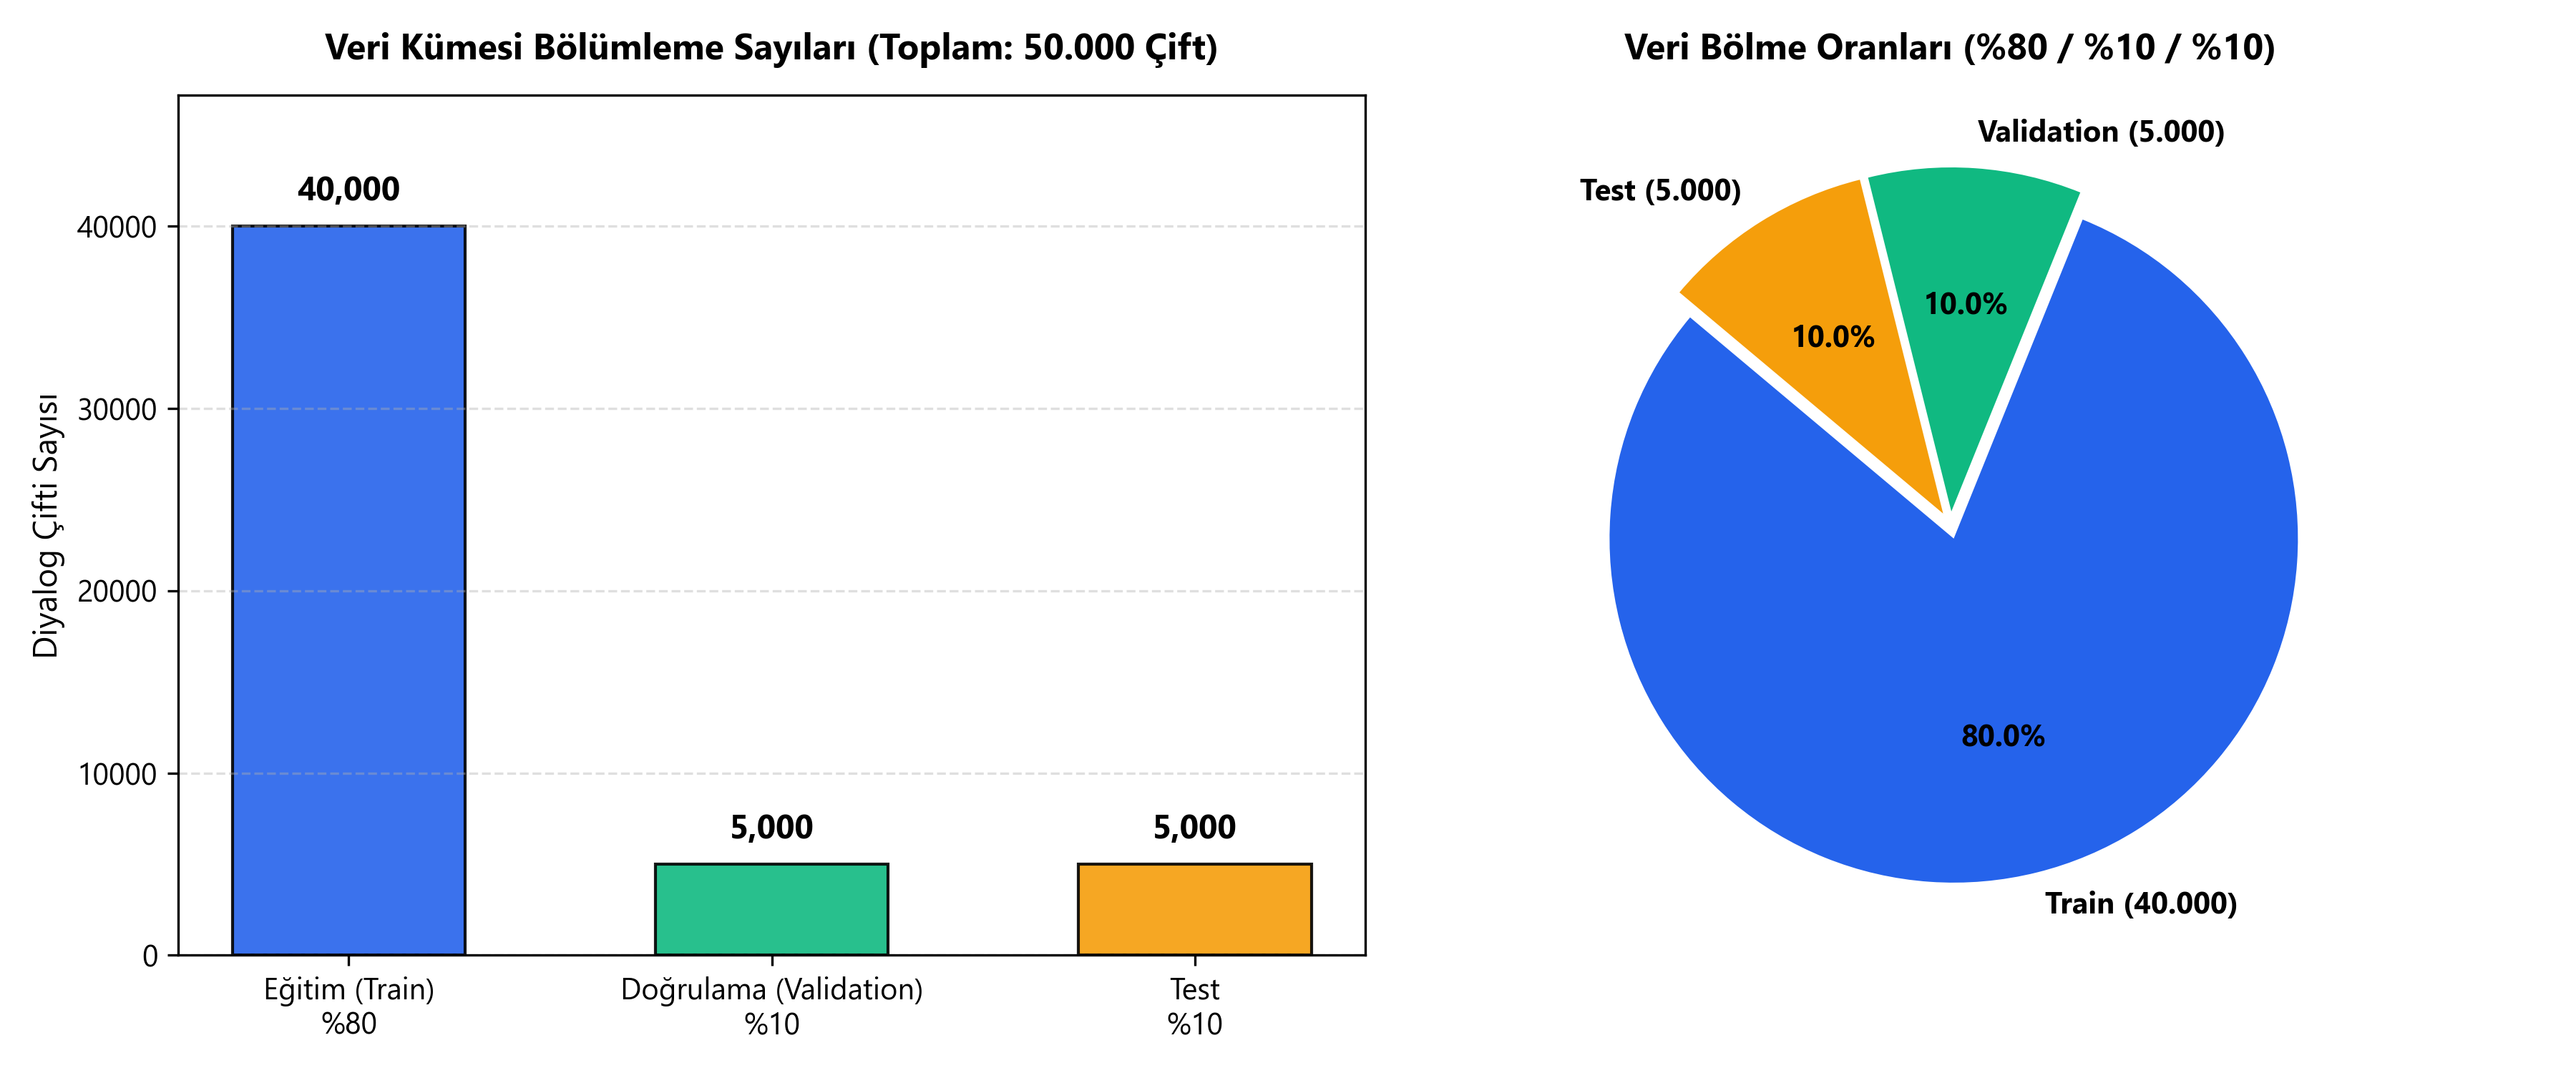
\includegraphics[width=0.98\textwidth]{01_veri_bolumleme_split.png}
        \end{column}
    \end{columns}
\end{frame}

% --- SLAYT 5: Keşifsel Veri Analizi (EDA) ---
\begin{frame}{III. Keşifsel Veri Analizi (EDA): Uzunluk ve Kaynak Dağılımı}
    \begin{columns}[c]
        \begin{column}{0.52\textwidth}
            \centering
            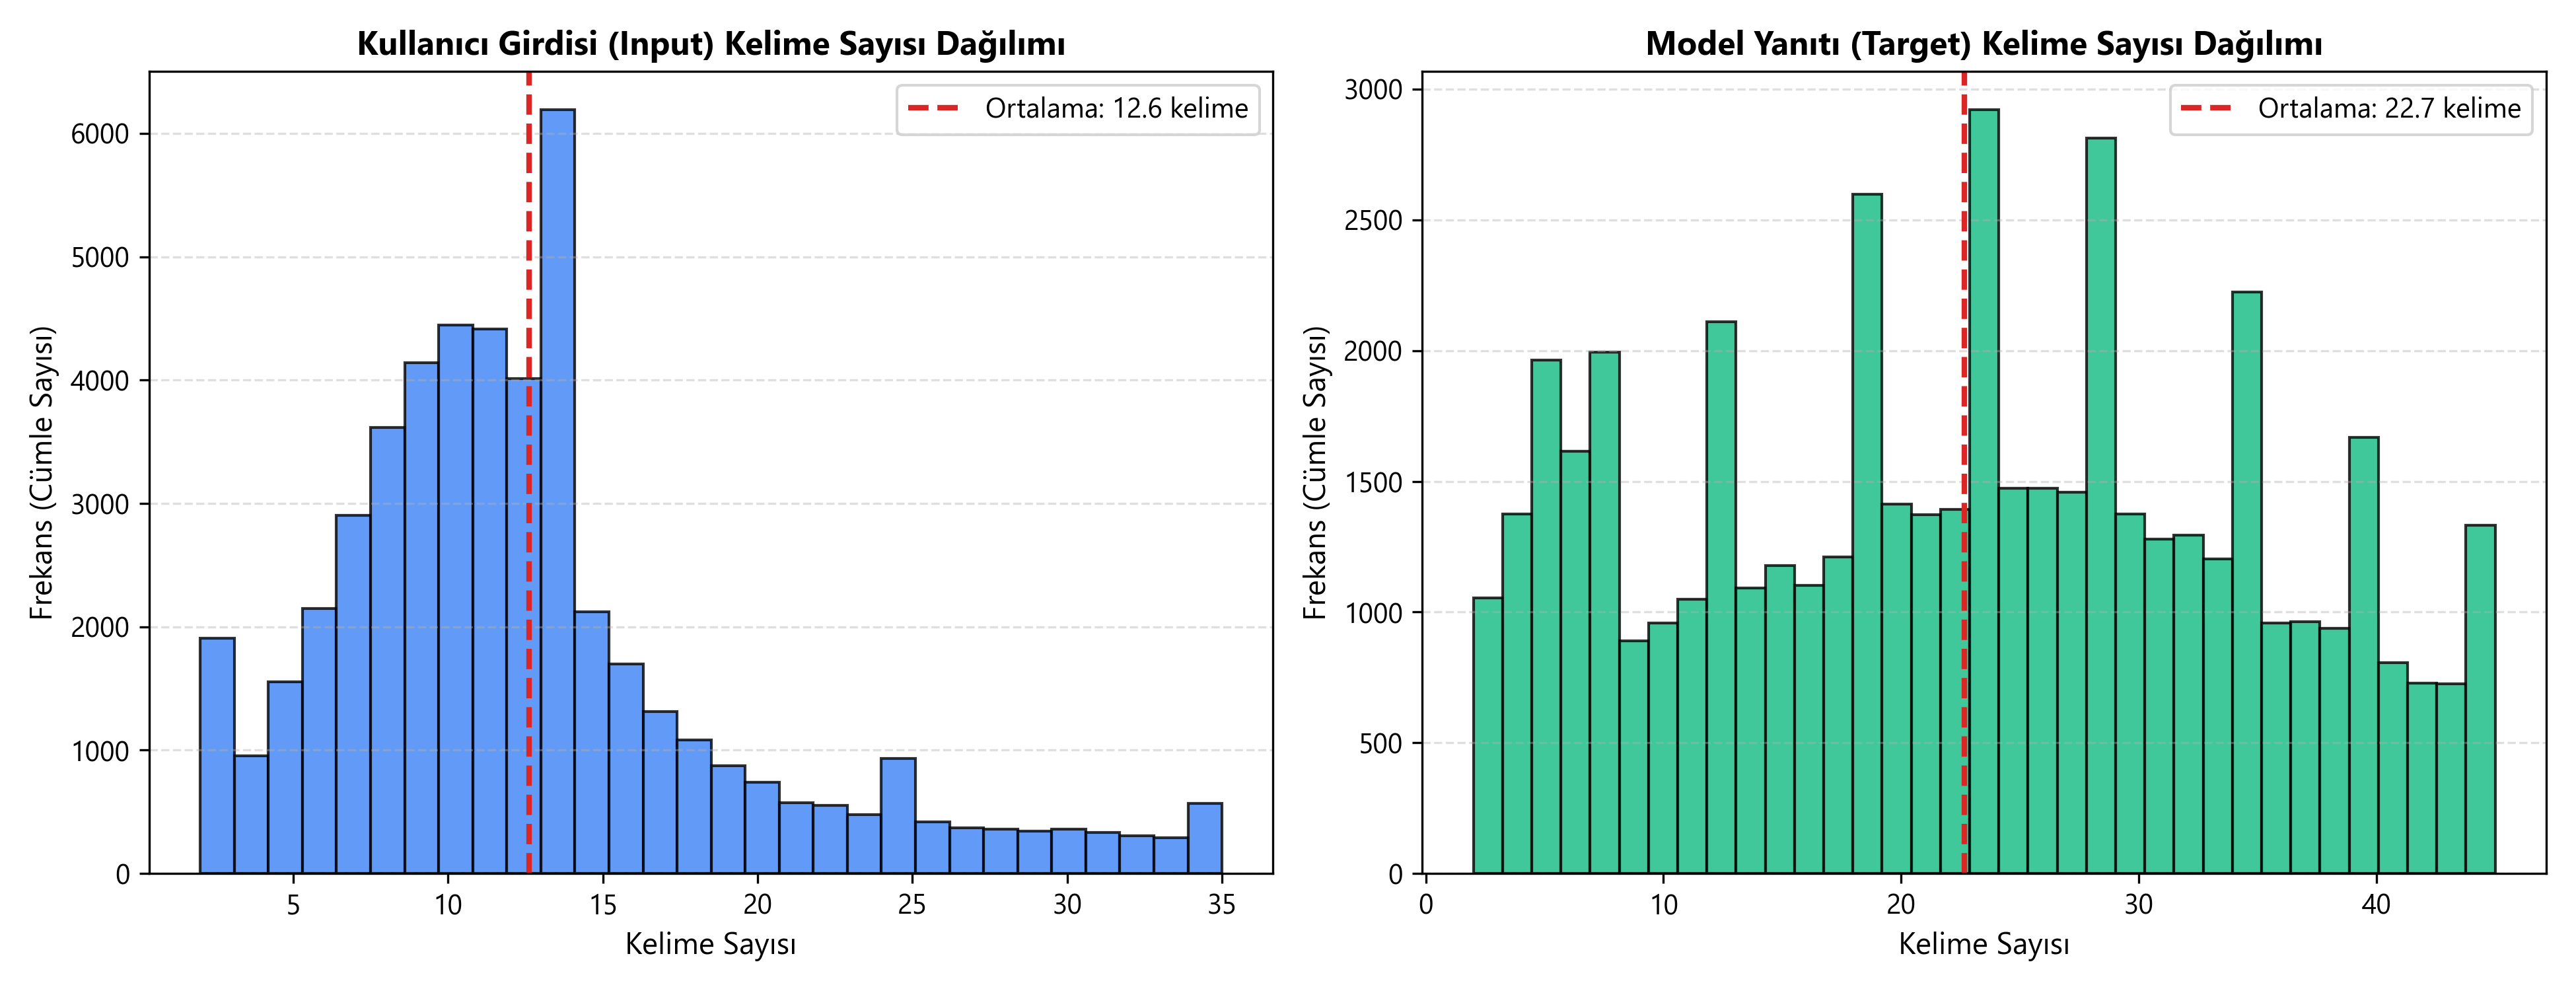
\includegraphics[width=0.98\textwidth]{02_kelime_uzunlugu_dagilimi.png}
            \vspace{2pt}
            {\scriptsize Ortalama Girdi: \textbf{9.73 kelime} $\mid$ Ortalama Yanıt: \textbf{15.49 kelime}}
        \end{column}
        \begin{column}{0.46\textwidth}
            \centering
            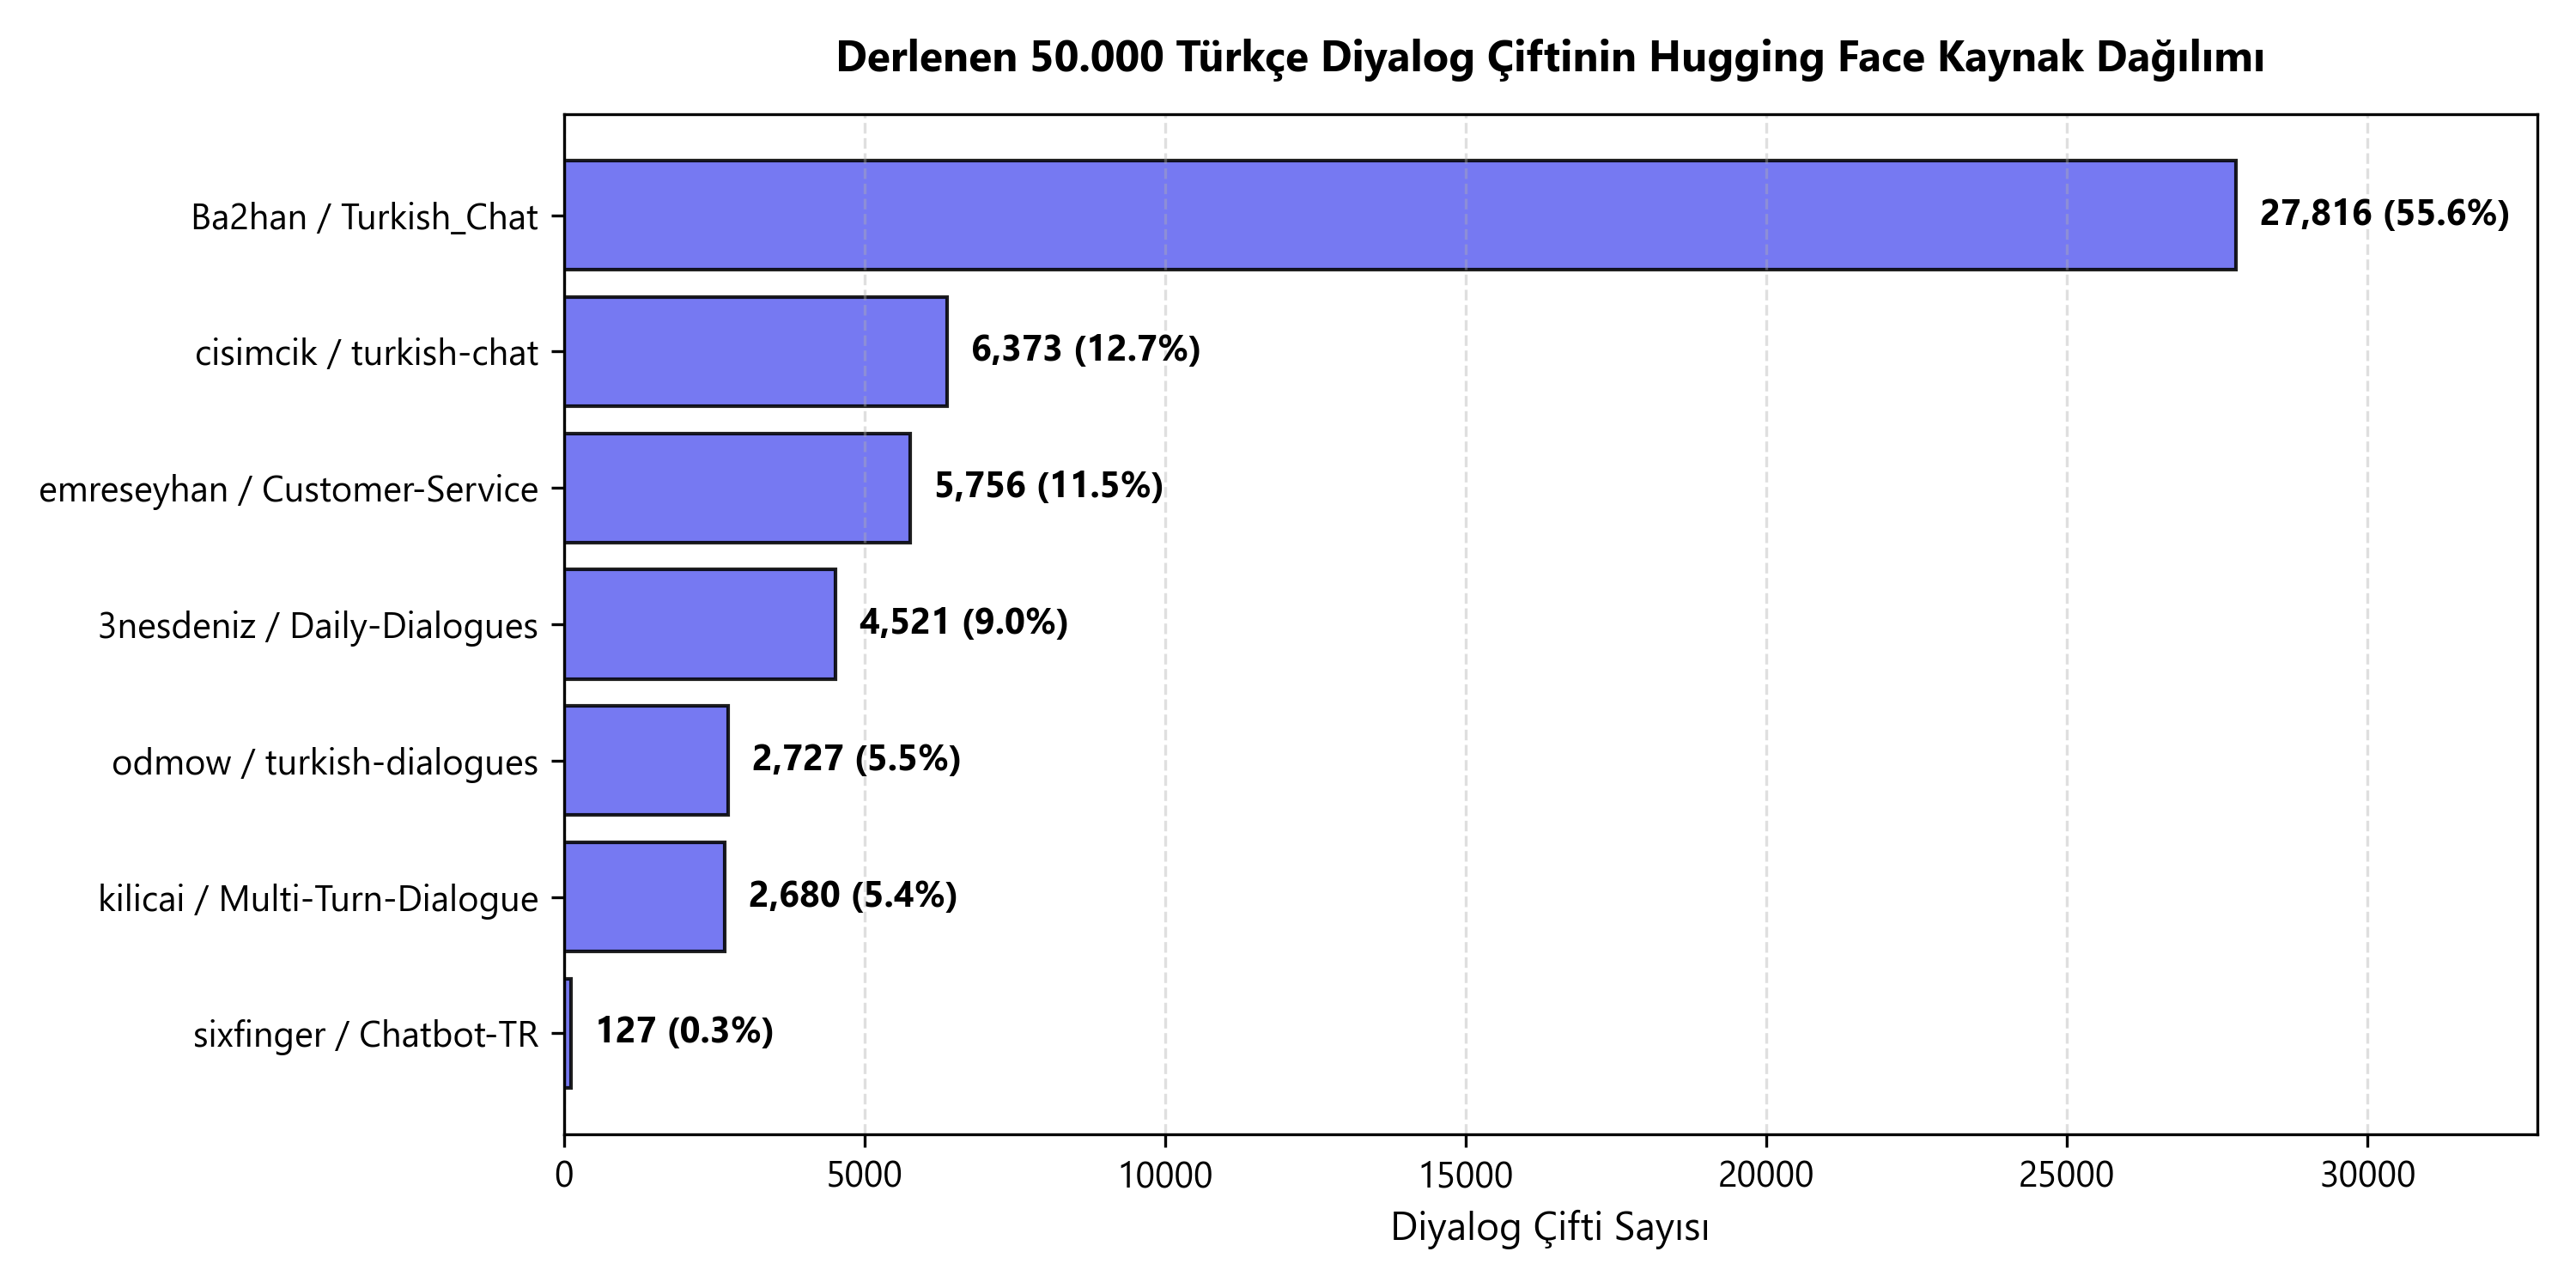
\includegraphics[width=0.98\textwidth]{03_veri_kaynaklari_dagilimi.png}
            \vspace{2pt}
            {\scriptsize Çoklu açık kaynak birleşimi ile yüksek alan çeşitliliği}
        \end{column}
    \end{columns}
\end{frame}

% --- SLAYT 6: Metodoloji ve Mimariler ---
\begin{frame}{IV--VI. Metodoloji ve Karşılaştırılan Derin Öğrenme Modelleri}
    \begin{columns}[T]
        \begin{column}{0.48\textwidth}
            \begin{block}{Baseline: 2-Katmanlı Seq2Seq Bi-LSTM}
                \begin{itemize}
                    \item \textbf{Parametre:} 23.1 Milyon (Sıfırdan Eğitim)
                    \item \textbf{Encoder:} 2 katmanlı Çift Yönlü LSTM ($d_{\text{emb}}=256, d_{\text{hid}}=256$, BPE 12k)
                    \item \textbf{Bahdanau (Additive) Attention:}
                    \[
                        e_{tj} = v_a^\top \tanh(W_a s_{t-1} + U_a h_j)
                    \]
                    \item \textbf{Decoder:} 2 katmanlı LSTM + Teacher Forcing ($0.5$)
                \end{itemize}
            \end{block}
        \end{column}
        \begin{column}{0.48\textwidth}
            \begin{block}{Model 1: Fine-Tuned Turkish-GPT-2}
                \begin{itemize}
                    \item \textbf{Parametre:} 124.4 Milyon (\texttt{gpt2-turkish-cased})
                    \item \textbf{Mimari:} 12 Katman, 12 Head, $d_{\text{model}}=768$, Resmi BPE (50.258 token)
                    \item \textbf{Causal Self-Attention:}
                    \[
                        \text{Attention}(Q,K,V) = \text{softmax}\!\left(\frac{QK^\top}{\sqrt{d_k}} + M\right)\!V
                    \]
                    \item \textbf{Eğitim:} \texttt{AdamW} ($\text{lr}=5\times10^{-5}$), \texttt{FP16}, Yalnızca \texttt{Asistan:} yanıtında Loss ($-100$ maskeleme)
                \end{itemize}
            \end{block}
        \end{column}
    \end{columns}
\end{frame}

% --- SLAYT 7: Baseline Eğitim Sonuçları ---
\begin{frame}{V. Baseline Model (Seq2Seq Bi-LSTM) Eğitim Analizi}
    \begin{columns}[c]
        \begin{column}{0.38\textwidth}
            \begin{block}{RTX 4060 GPU (5 Epoch)}
                \begin{itemize}
                    \item \textbf{Epoch 1:} Val Loss \texttt{7.6912} (PPL: \texttt{2188.9})
                    \item \textbf{Epoch 3:} Val Loss \texttt{7.3893} (PPL: \texttt{1618.6})
                    \item \textbf{Epoch 5:} Val Loss \textbf{\texttt{7.1915}} (PPL: \textbf{\texttt{1328.0}})
                    \item \textbf{Çıkarım Hızı:} \texttt{30.07 ms}
                    \item \textbf{Gözlem:} Sıfırdan eğitilen Bi-LSTM kaybı düşürse de yüksek Perplexity nedeniyle karmaşık cümlelerde zorlanmaktadır.
                \end{itemize}
            \end{block}
        \end{column}
        \begin{column}{0.60\textwidth}
            \centering
            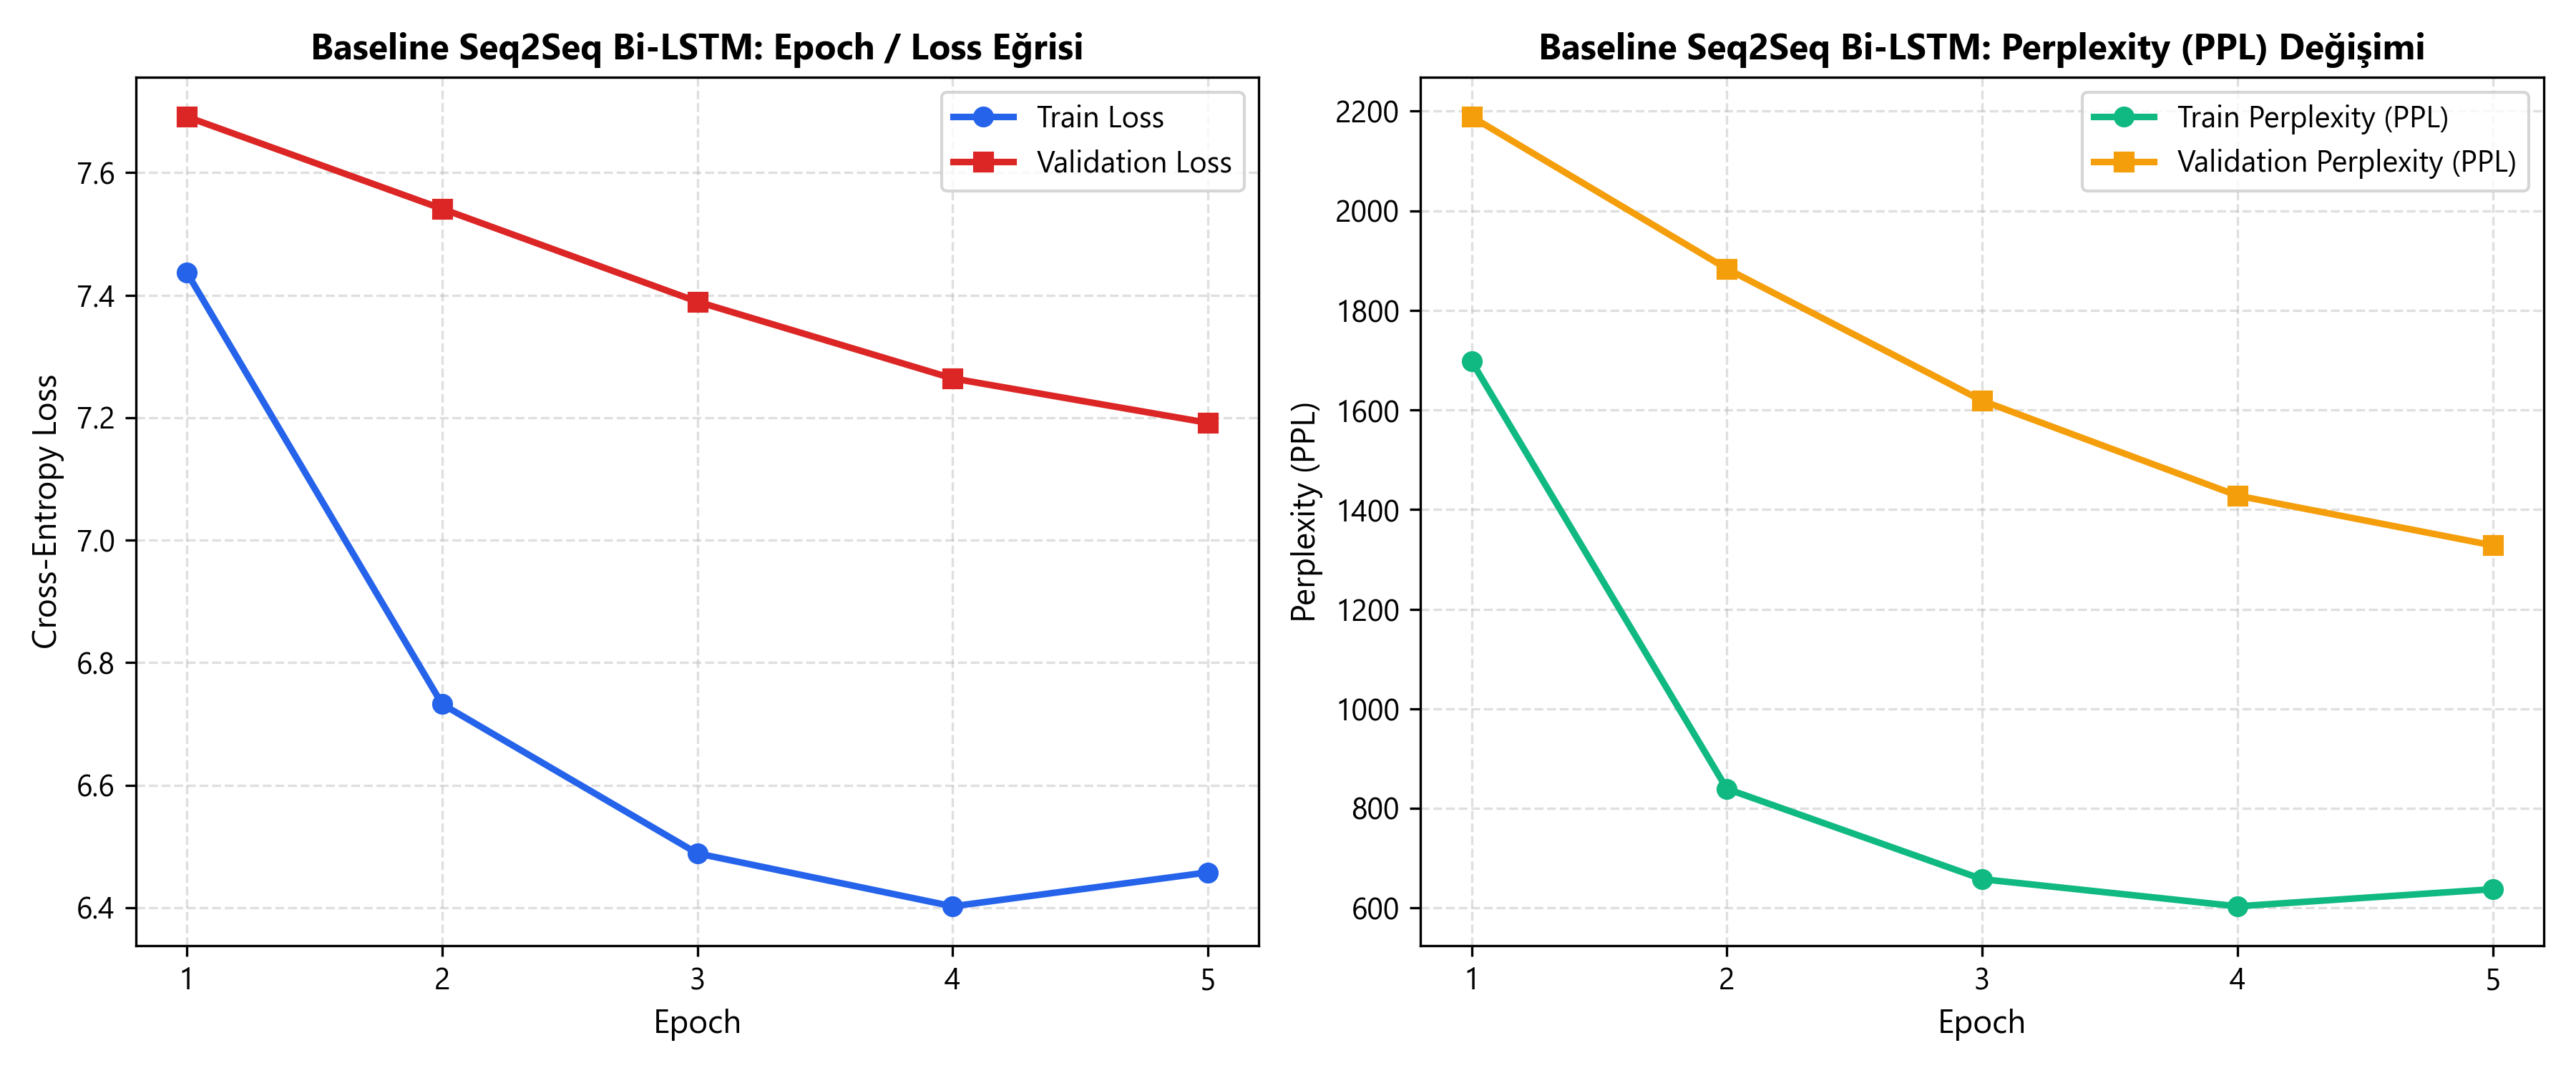
\includegraphics[width=0.99\textwidth]{04_baseline_lstm_egitim_egrisi.png}
        \end{column}
    \end{columns}
\end{frame}

% --- SLAYT 8: Karşılaştırmalı Loss ve Perplexity ---
\begin{frame}{VII. Deneysel Karşılaştırma: Validation Loss ve Perplexity (PPL)}
    \begin{columns}[c]
        \begin{column}{0.38\textwidth}
            \begin{block}{Transfer Öğrenme Etkisi}
                \begin{itemize}
                    \item \textbf{Validation Loss:} \texttt{7.1915} $\rightarrow$ \textbf{\texttt{3.4666}} (\textbf{\%51.8 azalma})
                    \item \textbf{Validation Perplexity:} \texttt{1328.04} $\rightarrow$ \textbf{\texttt{32.03}} (\textbf{41.5 kat iyileşme!})
                    \item Önceden eğitilmiş Türkçe dil temsilleri, modelin kelime tahmin belirsizliğini dramatik biçimde düşürmüştür.
                \end{itemize}
            \end{block}
        \end{column}
        \begin{column}{0.60\textwidth}
            \centering
            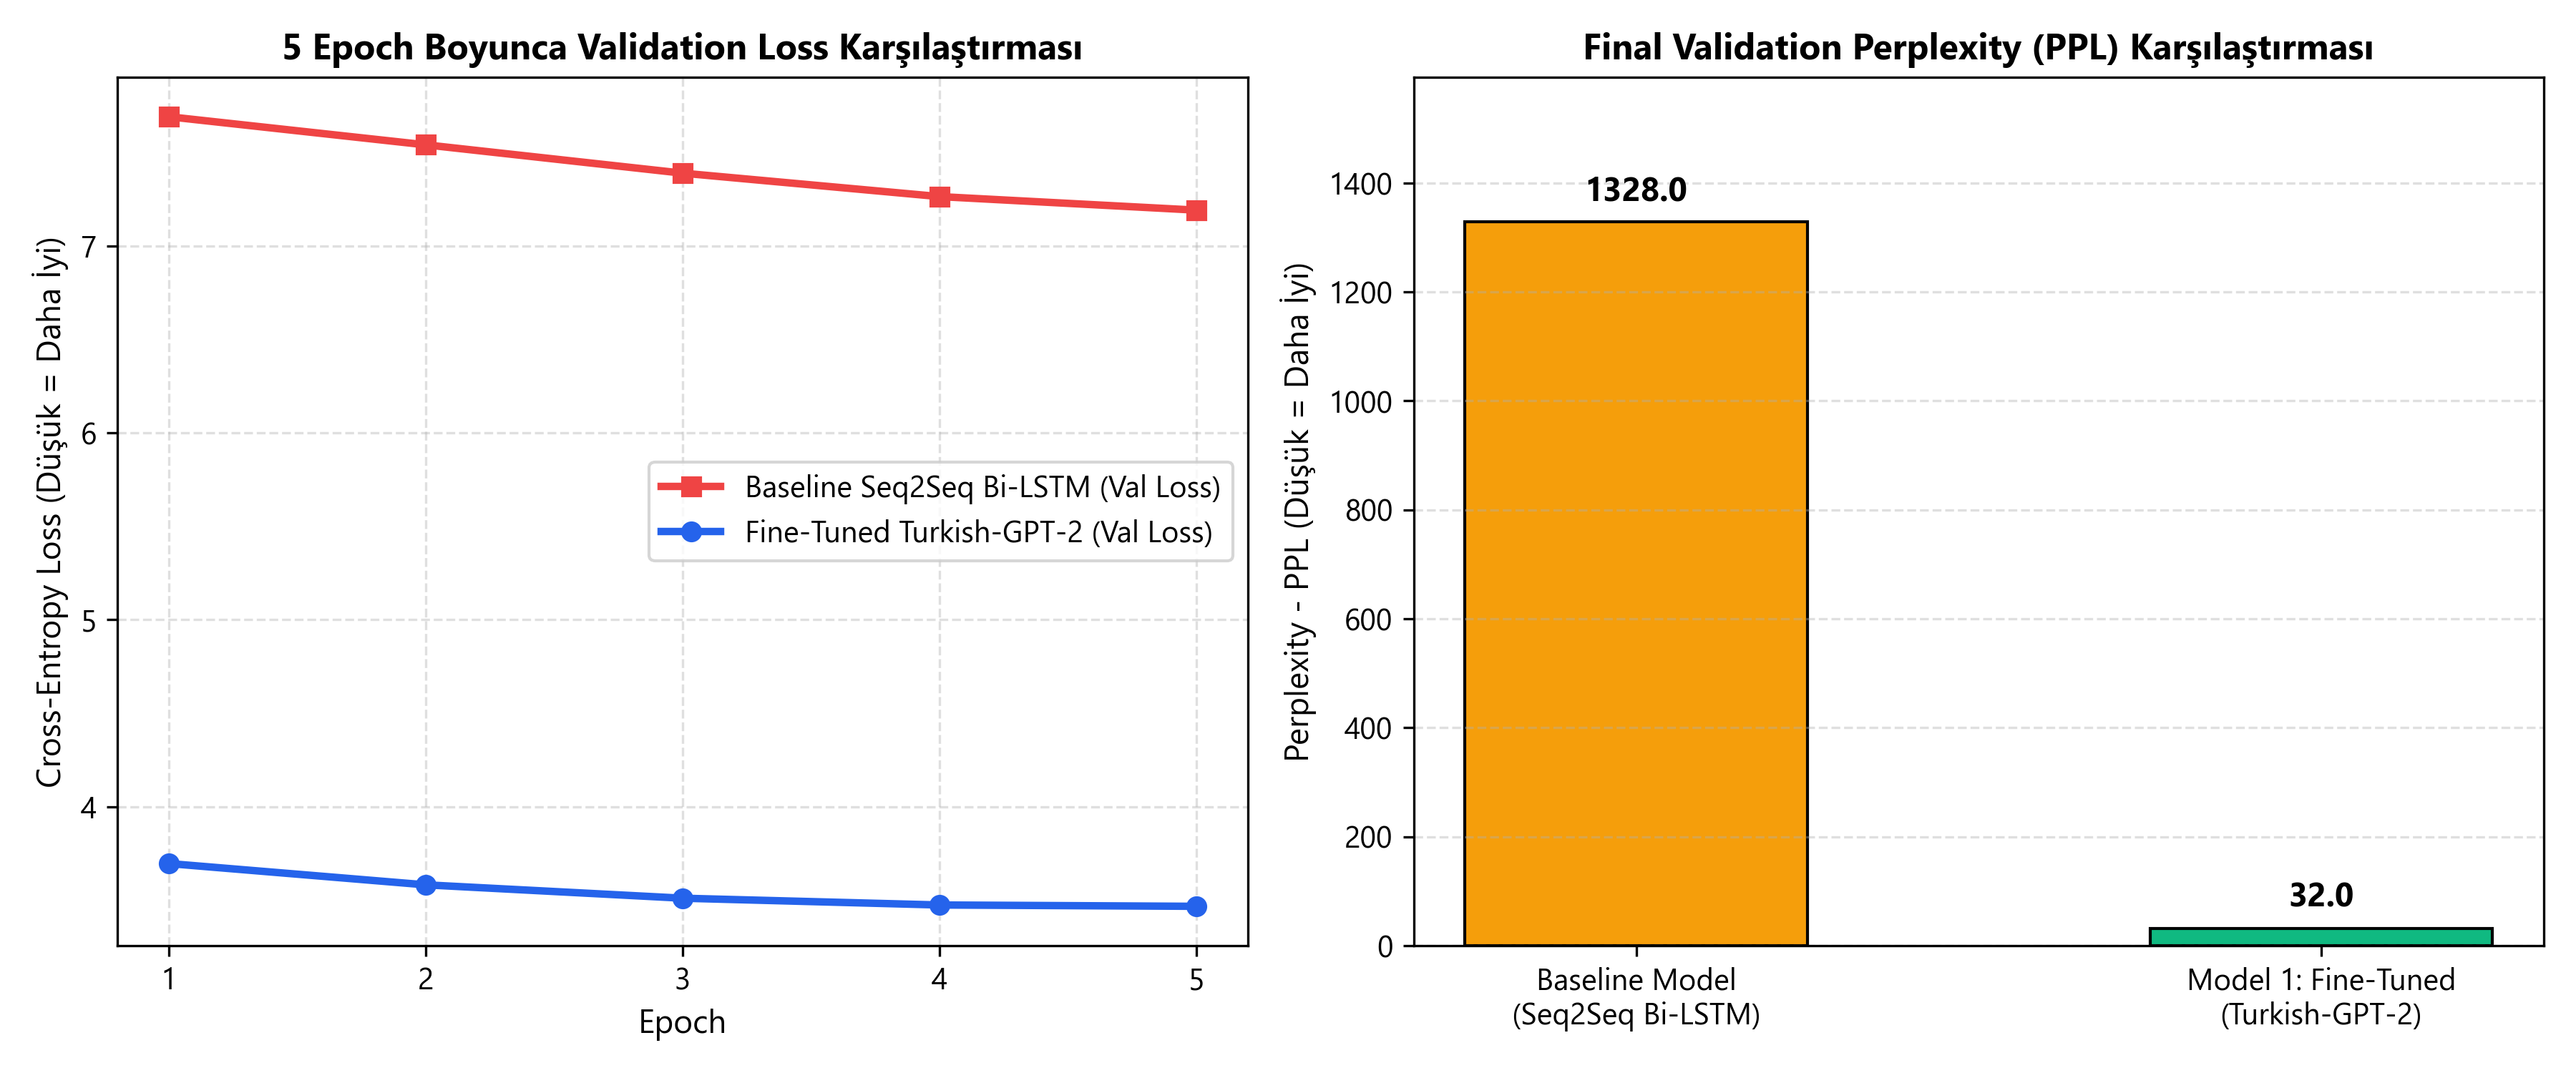
\includegraphics[width=0.99\textwidth]{05_model_karsilastirma_loss_ppl.png}
        \end{column}
    \end{columns}
\end{frame}

% --- SLAYT 9: BLEU, ROUGE ve Çıkarım Gecikmesi (Latency) ---
\begin{frame}{VII. Deneysel Karşılaştırma: BLEU, ROUGE ve Inference Latency}
    \begin{columns}[c]
        \begin{column}{0.38\textwidth}
            \begin{block}{Metin Kalitesi ve Hız Dengesi}
                \begin{itemize}
                    \item \textbf{BLEU-1:} \texttt{6.96} $\rightarrow$ \textbf{\texttt{10.60}} (\textbf{+\,\%52.3})
                    \item \textbf{BLEU-2:} \texttt{4.02} $\rightarrow$ \textbf{\texttt{5.70}} (\textbf{+\,\%41.8})
                    \item \textbf{ROUGE-1:} \texttt{9.76} $\rightarrow$ \textbf{\texttt{15.89}} (\textbf{+\,\%62.8})
                    \item \textbf{ROUGE-L:} \texttt{9.76} $\rightarrow$ \textbf{\texttt{14.47}} (\textbf{+\,\%48.3})
                    \item \textbf{Latency:} \texttt{352.9 ms} (\texttt{FP16 + KV-Cache} ile gerçek zamanlı $<0.4$ sn yanıt)
                \end{itemize}
            \end{block}
        \end{column}
        \begin{column}{0.60\textwidth}
            \centering
            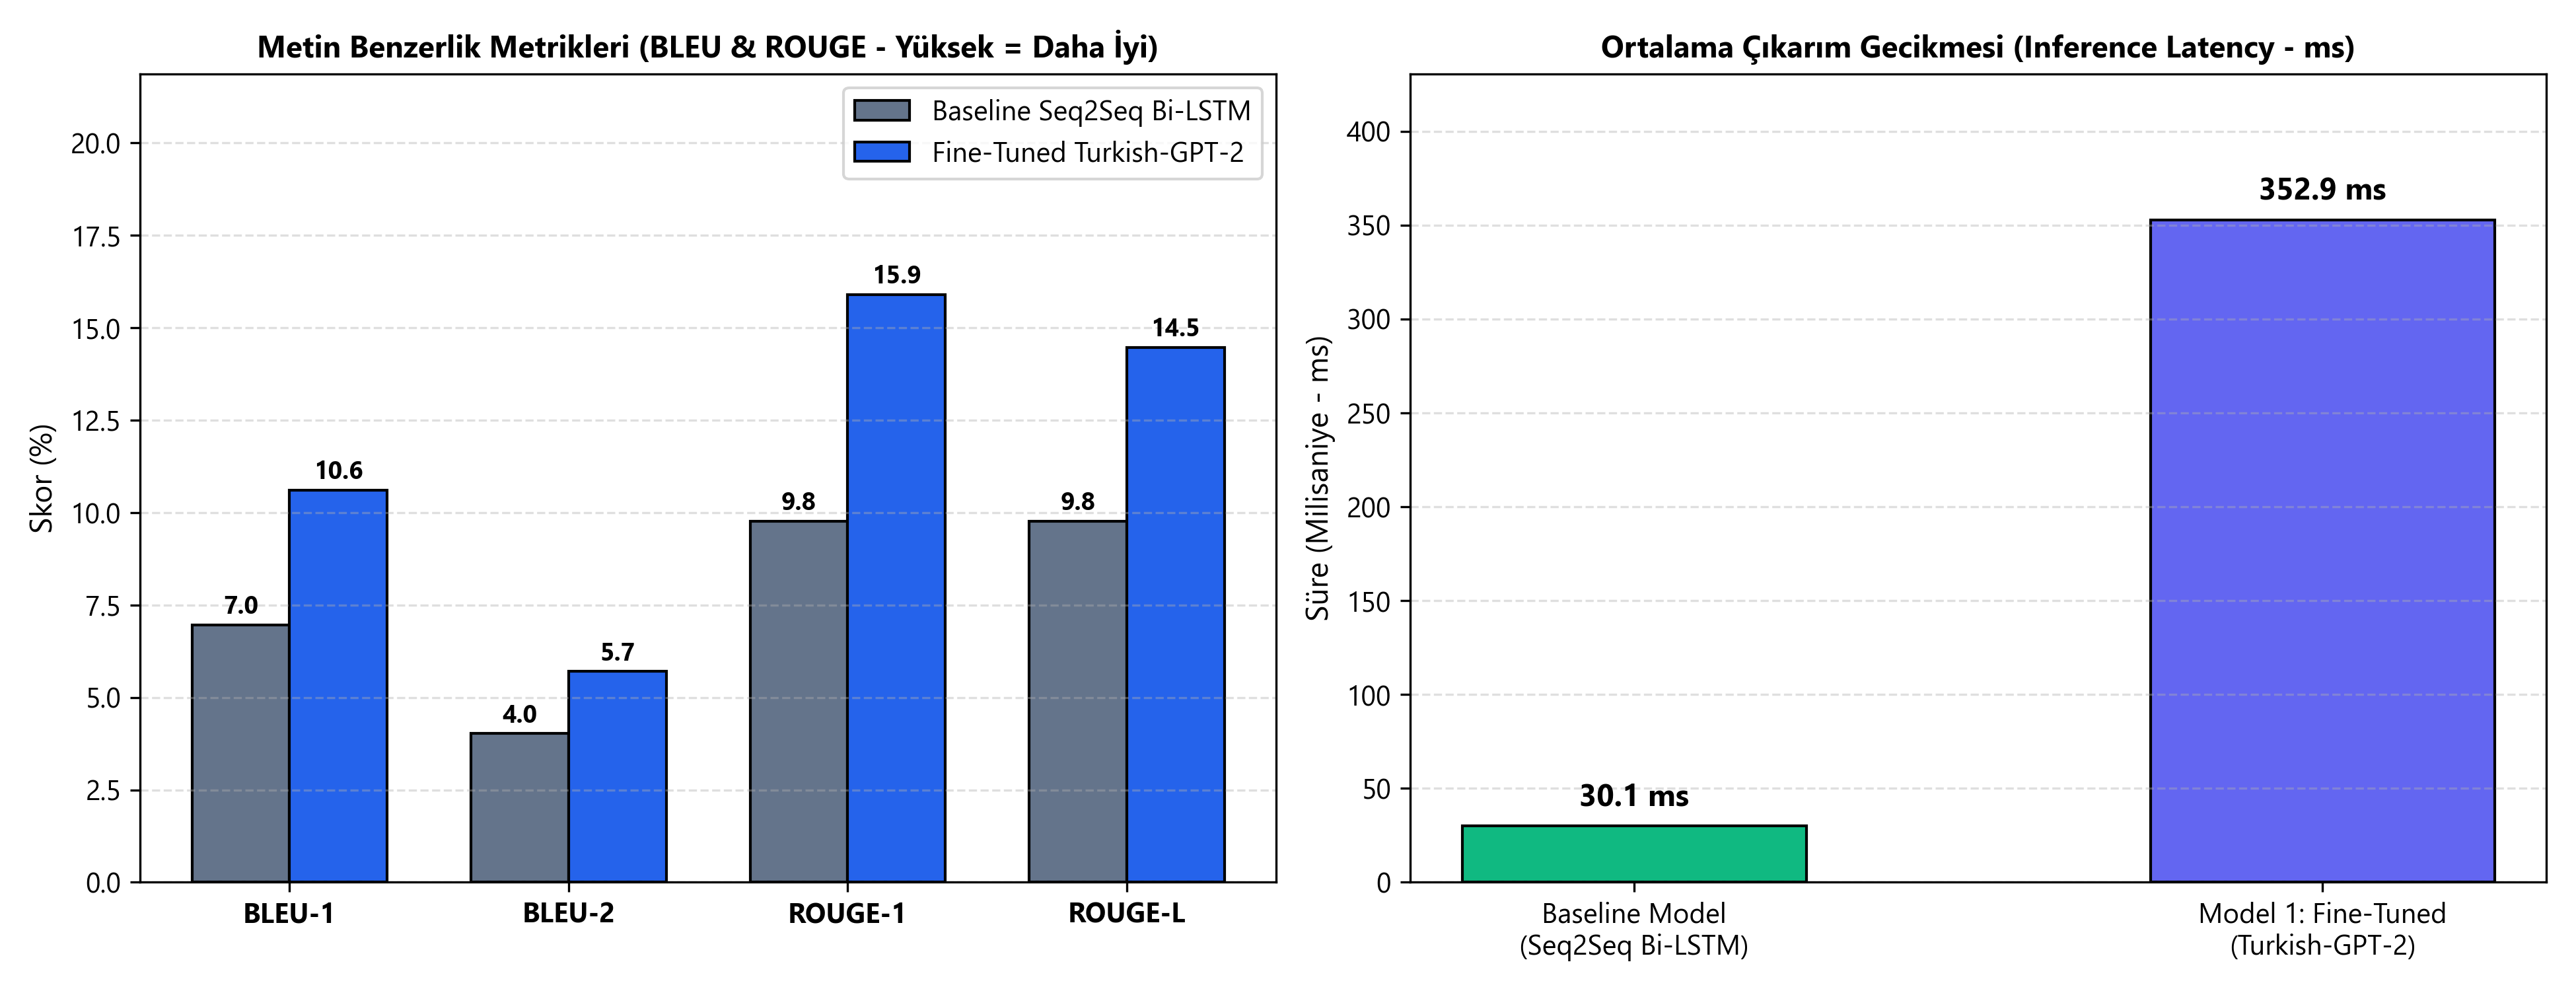
\includegraphics[width=0.99\textwidth]{06_metrik_ve_hiz_karsilastirmasi.png}
        \end{column}
    \end{columns}
\end{frame}

% --- SLAYT 10: Tüm Metrikler Özet Tablosu ve Niteliksel Örnekler ---
\begin{frame}{VII. Nicel Karşılaştırma Tablosu ve Nitel Diyalog Örnekleri}
    \begin{table}
        \centering
        \resizebox{0.96\textwidth}{!}{%
        \begin{tabular}{lccccccc}
            \toprule
            \textbf{Model} & \textbf{Parametre} & \textbf{Val Loss $\downarrow$} & \textbf{Val PPL $\downarrow$} & \textbf{BLEU-1 $\uparrow$} & \textbf{BLEU-2 $\uparrow$} & \textbf{ROUGE-1 $\uparrow$} & \textbf{Latency $\downarrow$} \\
            \midrule
            \textbf{Baseline Seq2Seq Bi-LSTM} & 23.1M & 7.1915 & 1328.04 & 6.96 & 4.02 & 9.76 & \textbf{30.07 ms} \\
            \textbf{Model 1: Fine-Tuned GPT-2} & 124.4M & \textbf{3.4666} & \textbf{32.03} & \textbf{10.60} & \textbf{5.70} & \textbf{15.89} & 352.90 ms \\
            \bottomrule
        \end{tabular}%
        }
    \end{table}
    \vspace{-4pt}
    \begin{block}{Niteliksel (Qualitative) Çıktı Analizi}
        \begin{itemize}
            \item \textbf{Girdi 1:} \textit{``Faturamda 'ödeme hatası' var. Ben ödeme yaptıktan sonra neden hala bu hatayı alıyorum?''}\\
            $\circ$ \textbf{Baseline Bi-LSTM:} \textit{Merhaba, yaşadığınız sorun için üzgünüz. Hemen kontrol ediyorum...}\\
            $\circ$ \textbf{Fine-Tuned GPT-2:} \textbf{\textit{Hesap numaranızı paylaşabilir misiniz?}}
            \item \textbf{Girdi 2:} \textit{``Enerji iç piyasalarındaki ilerlemeleri maddeler hâlinde anlat. Özellikle elektrik ve doğal gaz...''}\\
            $\circ$ \textbf{Baseline Bi-LSTM:} \textit{KİK, ve temel sorunlar şunlardır: 1. ve,: 1. ve,: 1. ve,: 1.} \textcolor{red}{(Darboğaz ve tekrar döngüsü)}\\
            $\circ$ \textbf{Fine-Tuned GPT-2:} \textbf{\textit{Enerji sektörü, enerji verimliliği gibi alanlarda önemli ilerlemeler kaydetmiştir. Enerji verimliliği ve yenilenebilir enerji kaynakları konusunda ise önemli adımlar atılmıştır.}}
        \end{itemize}
    \end{block}
\end{frame}

% --- SLAYT 11: Final Dönemi Yol Haritası ---
\begin{frame}{VIII. Sonuç ve Final Dönemi Yol Haritası (Model 2: LoRA / PEFT)}
    \begin{columns}[T]
        \begin{column}{0.48\textwidth}
            \begin{block}{Ara Sunuma Kadar Tamamlananlar ($\checkmark$)}
                \begin{itemize}
                    \item[$\checkmark$] 50.000 Türkçe diyalog çifti temizleme ve \%80/\%10/\%10 bölümleme
                    \item[$\checkmark$] Keşifsel Veri Analizi (EDA) ve BPE Tokenizasyon
                    \item[$\checkmark$] Baseline 2-Katmanlı Seq2Seq Bi-LSTM + Bahdanau Attention sıfırdan eğitimi
                    \item[$\checkmark$] Model 1 (\texttt{Turkish-GPT-2}) Full Fine-Tuning ve karşılaştırmalı metrik analizi
                \end{itemize}
            \end{block}
        \end{column}
        \begin{column}{0.48\textwidth}
            \begin{block}{Final Sunumu İçin Planlananlar ($\rightarrow$)}
                \begin{itemize}
                    \item[$\rightarrow$] \textbf{Model 2 (LoRA / PEFT İnce Ayar):} Düşük dereceli adaptasyon ($W_0 + \Delta W = W_0 + BA$, $r=16, \alpha=32$) ile parametrelerin yalnızca $\sim$\%1.2'sini eğiterek VRAM ve hız kazancı analizi
                    \item[$\rightarrow$] \textbf{3'lü Karşılaştırma:} Baseline Bi-LSTM vs. Full Fine-Tuning vs. LoRA Fine-Tuning
                    \item[$\rightarrow$] \textbf{Canlı Arayüz Demosu \& İnsan Değerlendirmesi}
                \end{itemize}
            \end{block}
        \end{column}
    \end{columns}
    \vspace{6pt}
    \centering
    \textbf{GitHub Deposu:} \url{https://github.com/sytali0/turkish-transformer-chatbot}
\end{frame}

\end{document}
